\documentclass[border=3pt,tikz]{standalone}
\usepackage{amsmath,amssymb}
\usepackage{tikz}
\tikzset{>=latex}

\colorlet{myblue}{black!50!blue}
\colorlet{mygreen}{black!50!green}
\colorlet{myred}{black!50!red}

\begin{document}


% RESISTANCE vs. TEMPERATURE
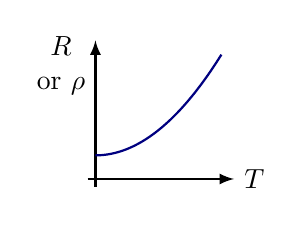
\begin{tikzpicture}
  \def\N{20}
  \def\xmin{-0.1} \def\xmax{1.6}
  \def\ymin{-0.1} \def\ymax{1.6}
  \draw[->,thick]
    (\xmin,0) -- (1.1*\xmax,0) node[right] {$T$};
  \draw[->,thick]
    (0,\ymin) -- (0,1.1*\ymax) node[above=5pt,below left,align=center] {$R$\\ or $\rho$};  
  \draw[thick,myblue,variable=\x,domain=0:\xmax,samples=\N,smooth]
    plot (\x,0.3+\x*\x/2);
\end{tikzpicture}


% PRESSURE vs. TEMPERATURE
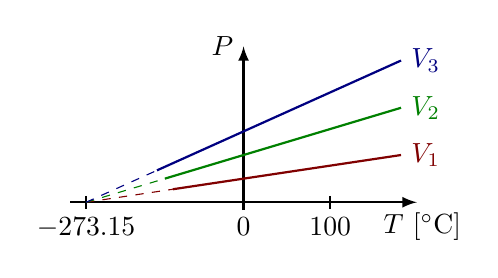
\begin{tikzpicture}
  \def\xmin{-2.0} \def\xmax{2.0}
  \def\ymin{-0.1} \def\ymax{1.8}
  \def\tick#1#2{\draw[thick] (#1+.08) --++ (0,-.16) node[below=-.5pt] {#2};}
  \def\ym#1#2{#1*\xmin,{#2*(#1*\xmin-\xmin)/(\xmax-\xmin)}}
  
  % AXIS
  \draw[->,thick]
    (1.1*\xmin,0) -- (1.1*\xmax,0) node[right=2,below] {$T$ [$^\circ$C]};
  \draw[->,thick]
    (0,\ymin) -- (0,1.1*\ymax) node[left,align=center] {$P$};
  
  % TICK
  \tick{\xmin,0}{$-273.15$}
  \tick{0,0}{0}
  \tick{1.1,0}{100}
  
  % GAS LINE
  \draw[thin,myred,dashed] (\xmin,0) -- (\ym{0.45}{0.6}) coordinate (V1);
  \draw[thick,myred] (V1) -- (\xmax,0.6) node[right] {$V_1$};
  \draw[thin,mygreen,dashed] (\xmin,0) -- (\ym{0.50}{1.2}) coordinate (V2);
  \draw[thick,mygreen] (V2) -- (\xmax,1.2) node[right] {$V_2$};
  \draw[thin,myblue,dashed] (\xmin,0) -- (\ym{0.55}{1.8}) coordinate (V3);
  \draw[thick,myblue] (V3) -- (\xmax,1.8) node[right] {$V_3$};
  
\end{tikzpicture}


% PRESSURE vs. VOLUME
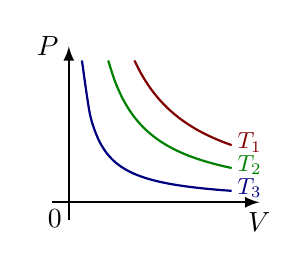
\begin{tikzpicture}
  \def\N{20}
  \def\nRTr{1.5}
  \def\nRTg{0.9}
  \def\nRTb{0.3}
  \def\xmax{2.2}
  \def\ymax{1.8}
  \def\tick#1#2{\draw[thick] (#1+.08) --++ (0,-.16) node[below=-.5pt] {#2};}
  
  % AXIS
  \draw[->,thick]
    (-0.1*\xmax,0) -- (1.1*\xmax,0) node[below] {$V$}; % [$\text{m}^3$]};
  \draw[->,thick]
    (0,-0.1*\xmax) -- (0,1.1*\ymax) node[left,align=center] {$P$};
  \node[below left=-1] at (0,0) {0};
  
  % ISOTHERMS
  \draw[thick,myred,variable=\x,domain=\nRTr/\ymax:0.94*\xmax,samples=\N,smooth]
    plot (\x,\nRTr/\x) node[above=1,right=-1,scale=0.84] {$T_1$};
  \draw[thick,mygreen,variable=\x,domain=\nRTg/\ymax:0.94*\xmax,samples=\N,smooth]
    plot (\x,\nRTg/\x) node[above=1,right=-1,scale=0.84] {$T_2$};
  \draw[thick,myblue,variable=\x,domain=\nRTb/\ymax:0.94*\xmax,samples=\N,smooth]
    plot (\x,\nRTb/\x) node[above=1,right=-1,scale=0.84] {$T_3$};
  
\end{tikzpicture}



\end{document}
